\section{Experiment 6 - Scalability}
\label{sec:exp6}
So far the experiments have been only executed on Dataset1 and the Healthcare dataset. In this experiment the Evo-RoleMiner$M$ is also applied on the Domino dataset (see Table \ref{tab:realDatasets}) and the average time needed for a generation is compared to experiments with the same settings with Dataset1 and the Healthcare dataset. The setup used can be seen in Table \ref{tab:exp4_setup}, where the generation size is set to 100  and the objectives "Confidentiality" and "Availability" are chosen for all experiments. An experiment on one dataset is executed 10 times. The specification of the machine, the experiments have been executed on, can be seen in Appendix \ref{sec:A_spec}.

\begin{figure}[H]
	\centering
	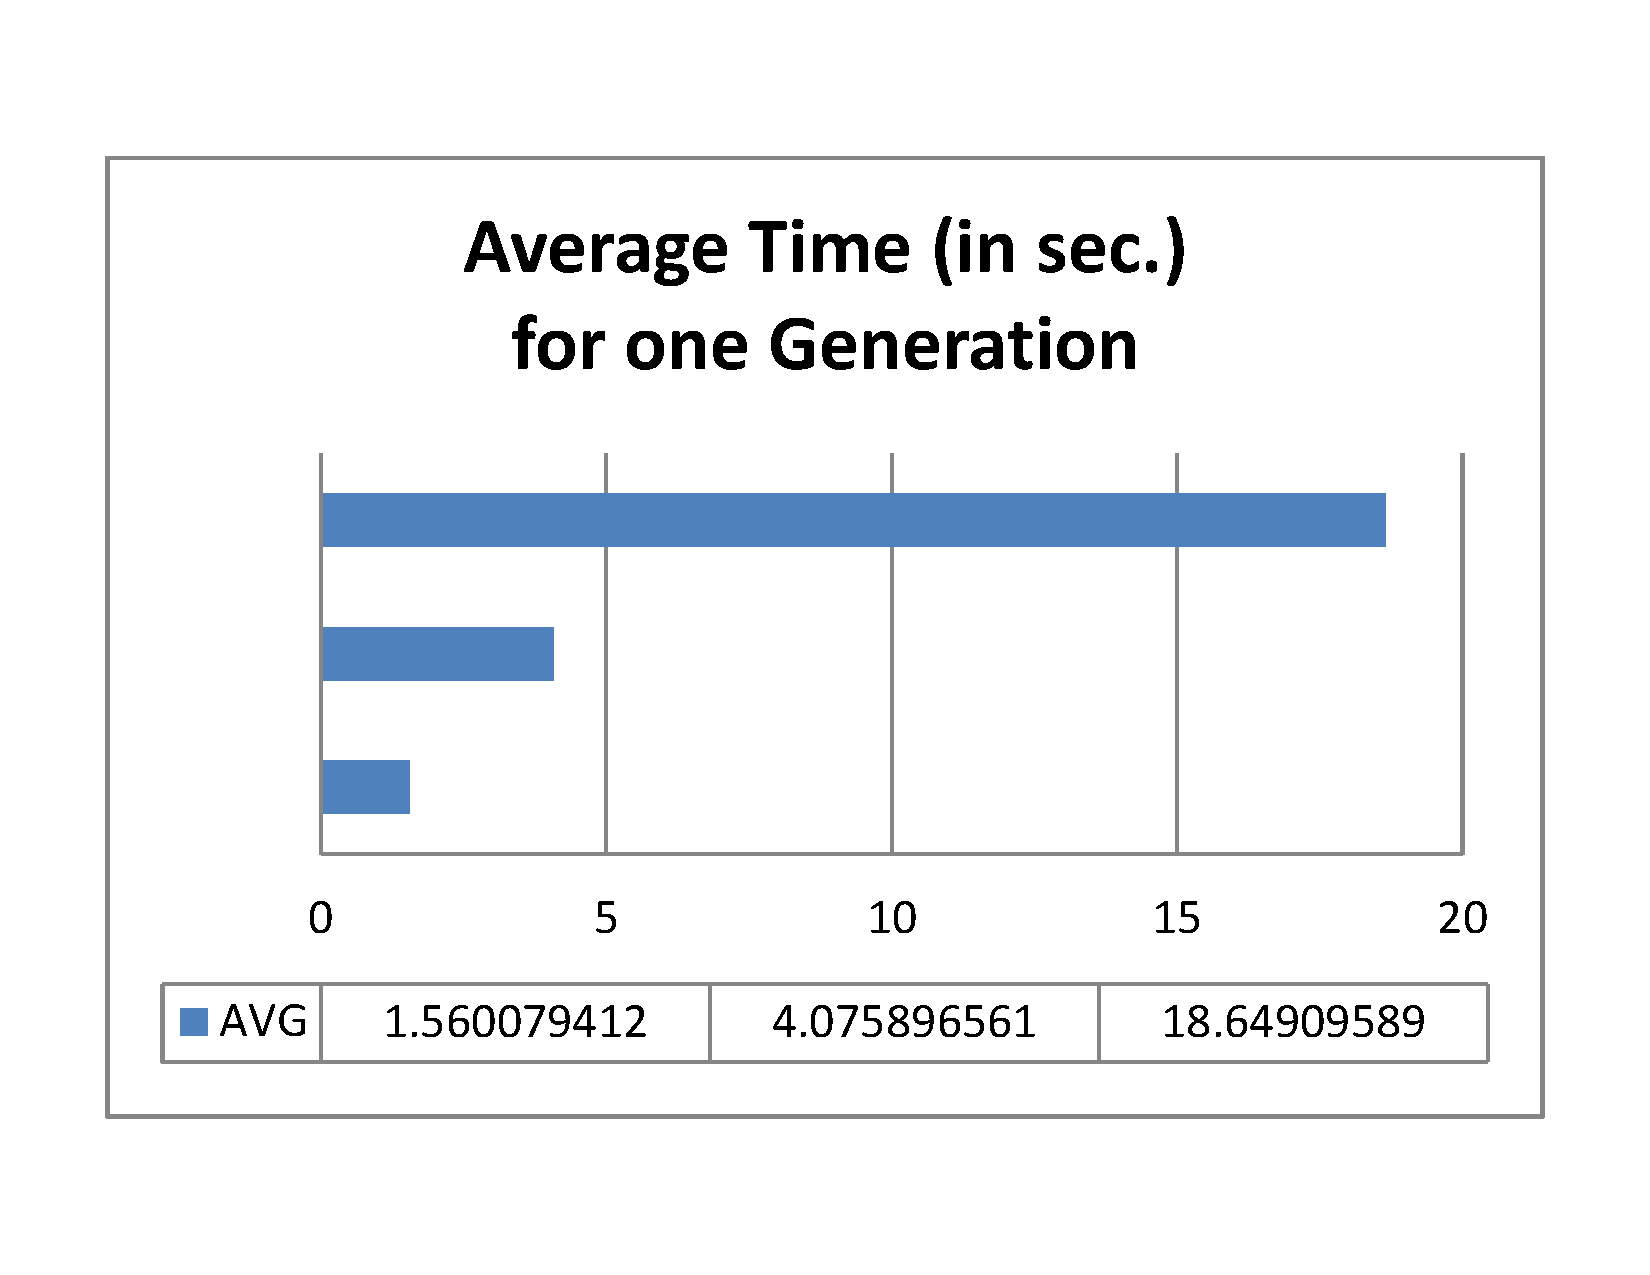
\includegraphics[width=0.6\textwidth]{Results_Exp6_Time}
	\caption{EXPERIMENT 6: Comparison of average time (in seconds) needed for a generation on Dataset1, Healthcare dataset and Domino dataset.}
	\label{fig:Results_Exp6_Time}
\end{figure}

 When applying the Evo-RoleMiner$M$ on the Domino dataset, the time needed for a generation quickly rises comapared to the smaller Dataset1 and the Healthcare dataset.